\chapter{A Simple GUI for the Hybrid NLP Element}

This chapter introduces a Graphical User Interface (GUI) developed as part of 
this work in order to 
facilitate analyses using the hybrid \acrshort{nlp} element. We detail the 
various features that are implemented using the AppDesigner utility of MATLAB, 
version 2022b. The chapter is divided in seven sections, each representing a 
particular tab of the interface. These seven tabs are : 1) Mesh, 2) Materials, 
3) Sections, 4) Boundary Conditions, 5) Analysis Controls, 6) Solve Job and, 
finally, 7) Post-processing. The first five tabs, some of which can be edited 
independently, belong to the pre-processing phase. Tab 6 calls the hybrid NLP 
solver for the given input in tabs 1-5 and tab seven provides post-processing 
infrormation with respect to the structure response in the form of 
force-displacement plots and  configuration history for all steps. A number of 
tooltips can be revealed by hovering over relevant fields.

\section{The Mesh Tab}

The first tab of the GUI, depicted in Fig. \ref{fig:TAB1_marked}, is concerned 
with nodal and element input. We analyze it in terms of parts A to M:

\begin{itemize}
	\item \textbf{A}: The Mesh tab.
	\item \textbf{B}: Facility used to manually add nodes. Numeric values 
	pertaining to the X (horizontal) and Y (vertical) coordinate axes are used 
	in the corresponding fields to define the coordinates of a node. By 
	clicking on the \textit{Add Node} button, the enumerated node is added to 
	the table with its coordinated also listed. The enumeration is automatic. 
	Attempting to add a node with coordinates (X,Y) that are already defined 
	for another node results in an error, as shown in Fig. 
	\ref{fig:TAB1_node_error}.
	\item \textbf{C}: Facility used to delete a particular node. The 
	\textit{Label} field takes as input the node label already generated and 
	removes it from the table. The enumeration of remaining nodes is updated 
	accordingly. If node deletion is performed after the mesh is generated, the 
	latter is no longer valid and all elements are removed.
	\item \textbf{D}: Success/Error indicator of an action pertaining to node 
	generation, coupled with a text field for relevant message output (e.g. see 
	\ref{fig:TAB1_node_error}).
	\item \textbf{E}: Facility to generate a node set from a \textbf{.txt} or 
	\textbf{.xlsx} file. The format for this input file is shown in Fig. 
	\ref{fig:TAB1_nodesfile}. If a number of nodes have already been added 
	manually, this action replaces all existing nodes. In contrast, generating 
	a nodal set from an input file and then manually adding additional nodes 
	results in appending the previously generated nodal list.
	\item \textbf{F}: Table that lists all generated nodes along with their 
	coordinates.
	\item \textbf{G}: Facility used to manually add a (hybrid \acrshort{nlp}) 
	beam element. Since only one element per member is adquate with the 
	proposed formulation, the only relevant inputs are the start and end node 
	labels, indicated in the relevant fields as \textit{Node} $i$ and 
	\textit{Node} $j$ respectively. Again, adding an element with start and end 
	nodes already defined for an existing element results in an error. In 
	addition, element enumeration is, again, automatic.
	\item \textbf{H}: Element deletion facility. The element label used as 
	input in the relevant field and by clicking the \textit{Delete Element} 
	button results in removal of the particular element from the table. The 
	remainig elements are, again, automatically re-enumerated.
	\item \textbf{I}: Success/Error indicator of an action pertaining to 
	element generation, coupled with a text field for relevant message output.
	\item \textbf{J}: Facility to generate an element partition from a 
	\textbf{.txt} or \textbf{.xlsx} file. The format for this input file is 
	shown in Fig. \ref{fig:TAB1_elementsfile}. If a number of elements have 
	already been added manually, this action replaces all existing elements. In 
	contrast, generating an element partition from an input file and then 
	manually adding additional elements results in appending the previously 
	generated element list.
	\item \textbf{K}:  Table that lists all generated elements along with their 
	start and end nodes.
	\item \textbf{L}: Once clicked, the \textit{Clear Mesh} button resets all 
	existing input in the Mesh tab and the user can start over.
	\item \textbf{M}: GUI axes that dynamically update the existing state of 
	nodal and mesh configuration. Figure \ref{fig:TAB1_mesh_example} shows the 
	Mesh tab when the mesh generation is complete for a simple case of a one 
	bay, one story frame. The nodal labels are places right next to their 
	respective nodes and are typeset in normal font while element labels are 
	approximately placed in the midspan of their corresponding elements and are 
	typeset in italic bold fonts.
\end{itemize}

\begin{figure}
	\centering
	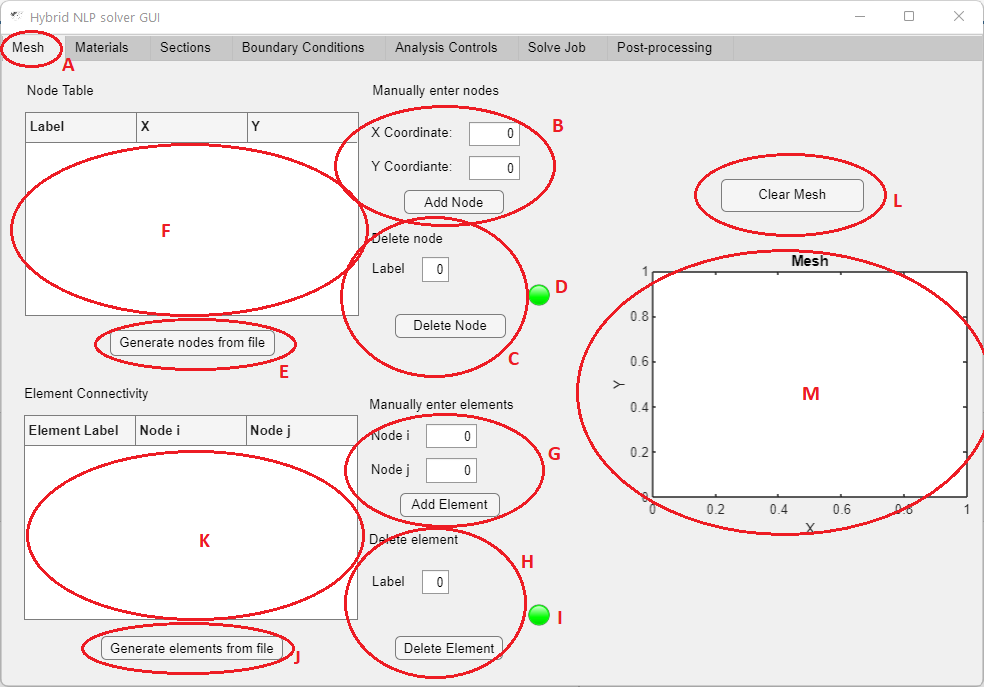
\includegraphics[scale=0.6]{GUIpics/TAB1/TAB1_marked.png}
	\caption{The \textit{Mesh} tab with relevant facilities A-M marked in red 
	circles 
	and enumerated with capital english letters.}
	\label{fig:TAB1_marked}
\end{figure}

\begin{figure}
	\centering
	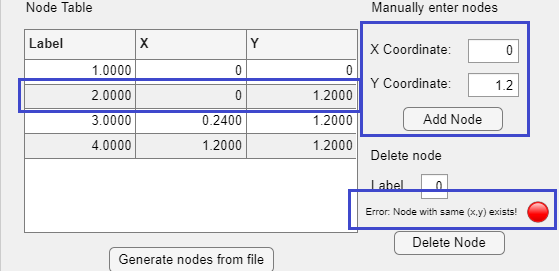
\includegraphics[scale=0.6]{GUIpics/TAB1/TAB1_node_error.png}
	\caption{Error when attempting to add a node with coordinates already 
	defined for an existing node.}
	\label{fig:TAB1_node_error}
\end{figure}

\begin{figure}
	\centering
	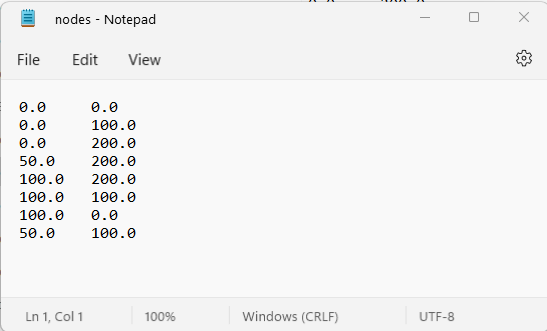
\includegraphics[scale=0.6]{GUIpics/TAB1/TAB1_nodesfile.png}
	\caption{A .txt file with the required format for nodal input. First column 
	is X coordinate, second is Y coordinate. The $k$-th row represents Node 
	$k$.}
	\label{fig:TAB1_nodesfile}
\end{figure}
\begin{figure}
	\centering
	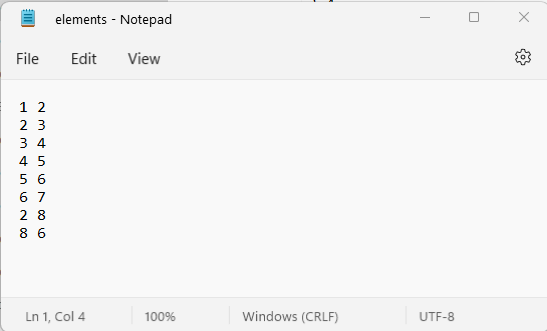
\includegraphics[scale=0.6]{GUIpics/TAB1/TAB1_elementsfile.png}
	\caption{A .txt file with the required format for element input. First 
	column is start node $i$, second is end node $j$. The $k$-th row represents 
	Element $k$.}
	\label{fig:TAB1_elementsfile}
\end{figure}

\begin{figure}
	\centering
	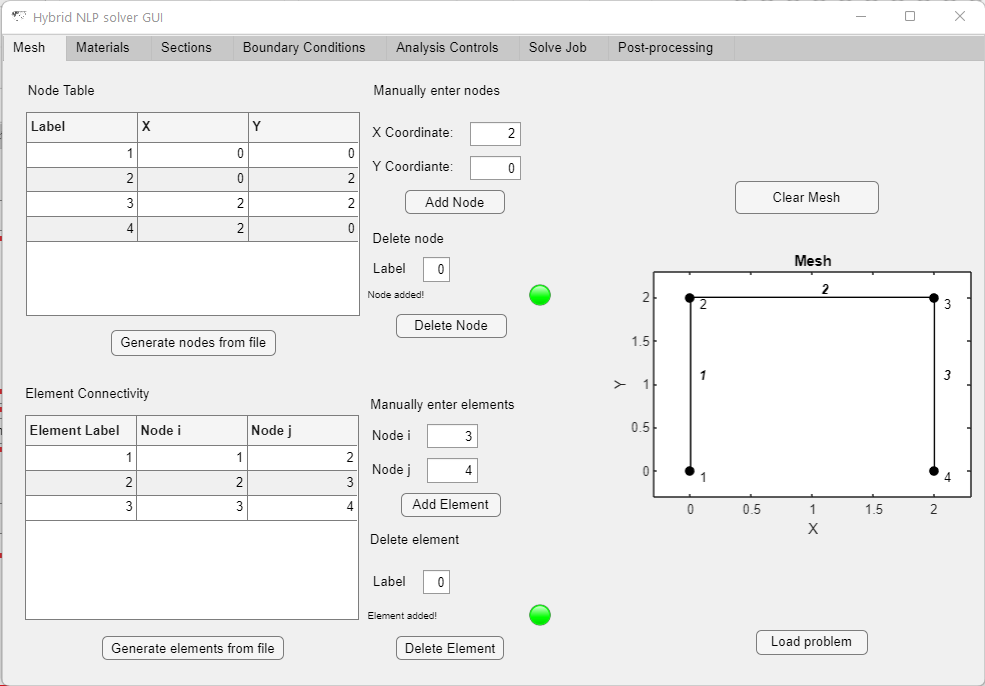
\includegraphics[scale=0.6]{GUIpics/TAB1/TAB1_mesh_example.png}
	\caption{The \textit{Mesh} tab with a completed mesh.}
	\label{fig:TAB1_mesh_example}
\end{figure}


\section{The Materials Tab}

The \textit{Materials} tab follows the \textit{Mesh} tab and does not have any 
dependencies regarding previous input. Figure FIG outlines all relevant fields 
in this tab, again, separated by red cycles based on their functionality. We 
list and describe items A-I below:

\begin{itemize}
	\item \textbf{A}: The \textit{Materials} tab.
	\item \textbf{B}: Material name field. Takes alphanumeric values. If a 
	material name is not specified, a default name \textbf{Material}\_$\#$ is 
	used, where $\#$ takes values 1,2,3... etc. As an example, see Fig. 
	\ref{fig:TAB2_adding_mat_noname}.
	\item \textbf{C}: Numeric fields pertaining to elastic and plastic 
	properties of the material. In the case of purely elastic analysis, dummy 
	or zero values can be used in the plastic fields, as they are not 
	considered.
	\item \textbf{D}: The \textit{Add} and \textit{Delete} material facilities, 
	along with the Success/Error indicator (green lamp icon). To delete a 
	material defined previously, the user needs to click on it in the 
	\textit{Materials Panel} seen on the left side of the tab (\textbf{Item H}, 
	see below), and then click the \textit{Delete} button.
	\item \textbf{E}: Axes that depict the uniaxial stress-strain law for a 
	defined material. In order to activate it, the user will need to click on 
	the specific material in the \textit{Materials Panel} seen on the left side 
	of the tab (\textbf{Item H}, see below). An max strain 
	$\epsilon_{max}=10\epsilon_y$ is specified purely for plotting purposes. 
	This feature can be seen in Fig. \ref{fig:TAB2_materials_added}.
	\item \textbf{F}: The \textit{Update Material} facility updates the elastic 
	and plastic properties of an existing material. The material to be updated 
	needs to be selected in the \textit{Materials panel} seen on the left side 
	of the tab (\textbf{Item H}, see below). 
	\item \textbf{G}: A \textit{Standard materials} facility, which is 
	introduced to quickly add predefined, standardized materials from the 
	drop-down list. These materials are assumed to be elastic-perfectly plastic 
	but can be modified using the \textit{Update Material} facility. Two 
	materials are available: 1) Structural Steel(S235) and 2) Aluminum 
	Alloy(6062) (see Fig \ref{fig:TAB2_predefined_mats}). In contrast with 
	manually adding materials, duplicate 
	materials from the drop-down are not permitted, as can be seen from Fig. 
	\ref{fig:TAB2_adding_already_predefmat}. 
	\item \textbf{H}: This is the \textit{Materials} panel. All materials 
	defined and added are listed here. The user needs to click on a specific 
	material on the list in order to i) delete it, ii) update its parameters or 
	iii) view its uniaxial stress-strain plot.
	\item \textbf{I}: The elastic and plastic properties of a material selected 
	on the \textit{Materials} panel are shown in this table. The tabulated 
	quantities correspond to the material fields in \textbf{B} as follows:
		i) $E$ represents Young's modulus, ii) $\nu$ represents Poisson's 
		ratio, iii) f\_y represents the yield stress of the material, iv) 
		$H_{iso}$ represents the isotropic hardening modulus and v) $H_{kin}$ 
		represents the kinematic hardening modulus.
\end{itemize}

\begin{figure}
	\centering
	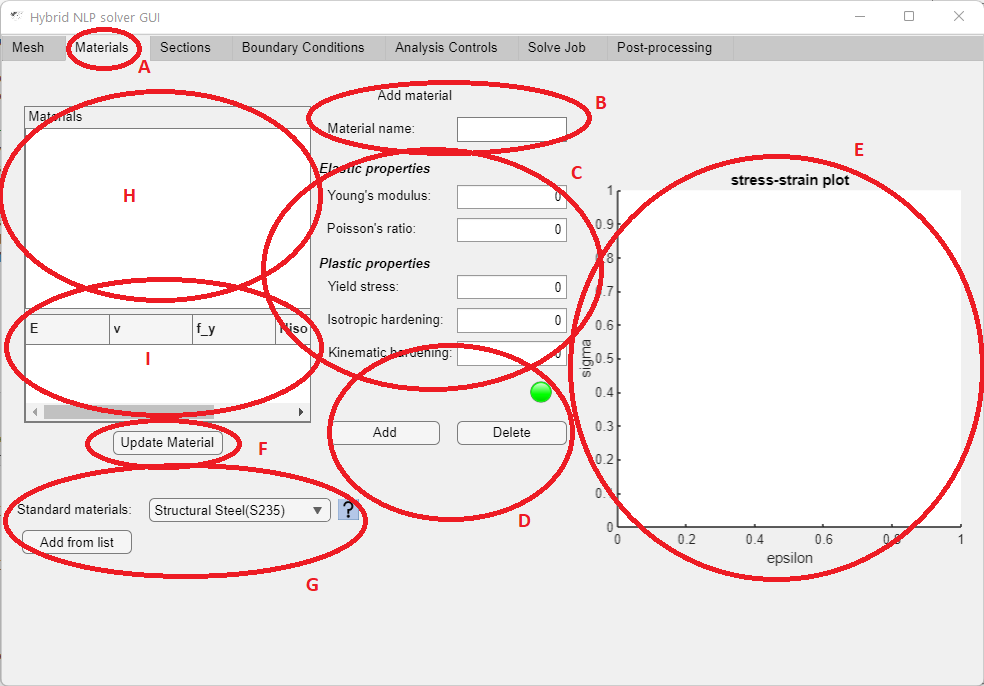
\includegraphics[scale=0.6]{GUIpics/TAB2/TAB2_marked.png}
	\caption{The \textit{Materials} tab with relevant facilities A-M marked in 
	red circles 
		and enumerated with capital english letters.}
	\label{fig:TAB2_marked}
\end{figure}


\begin{figure}
	\centering
	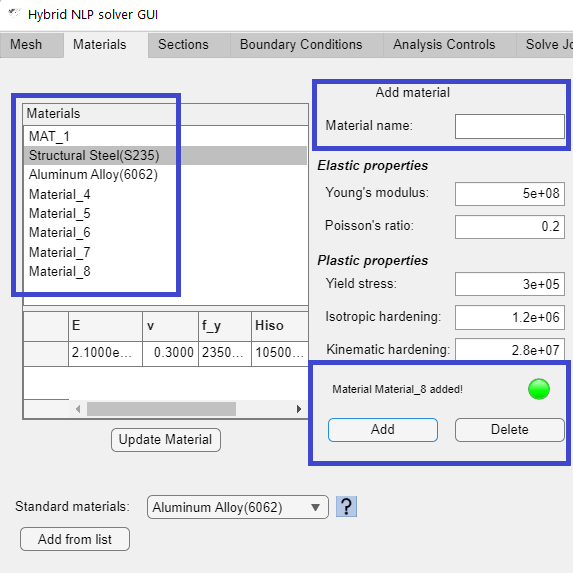
\includegraphics[scale=0.6]{GUIpics/TAB2/TAB2_adding_mat_noname.png}
	\caption{Multiple materials defined without a specified material name.}
	\label{fig:TAB2_adding_mat_noname}
\end{figure}

\begin{figure}
	\centering
	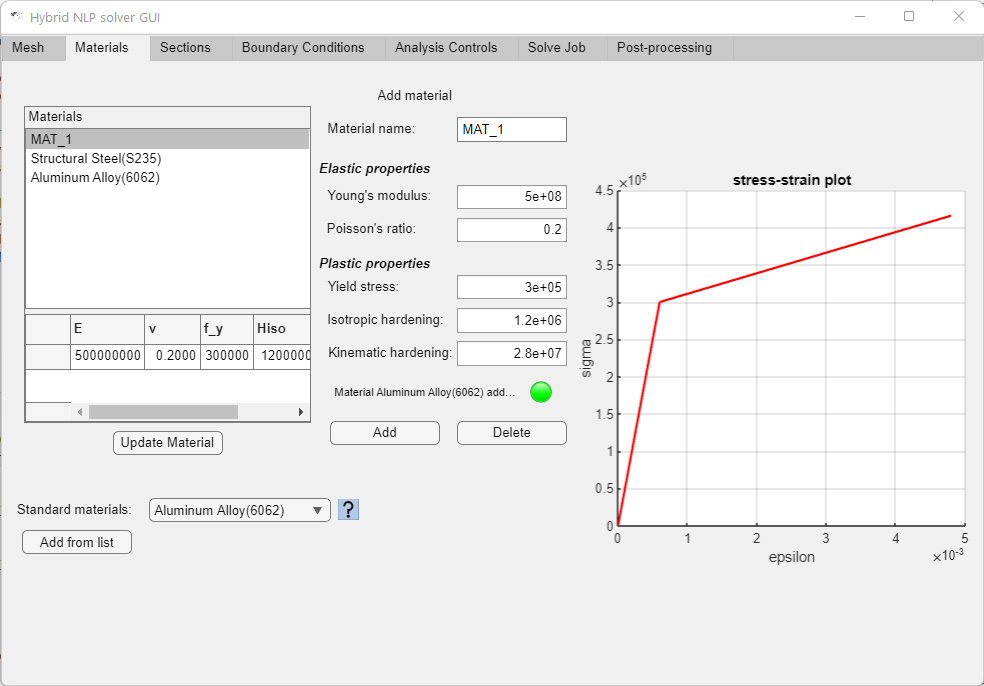
\includegraphics[scale=0.6]{GUIpics/TAB2/TAB2_materials_added.png}
	\caption{Potting of uniaxial stress-strain law of material \textbf{MAT}\_1.}
	\label{fig:TAB2_materials_added}
\end{figure}

\begin{figure}
	\centering
	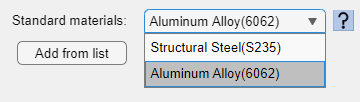
\includegraphics[scale=0.6]{GUIpics/TAB2/TAB2_predefined_mats.png}
	\caption{Available predefined materials from the \textit{Standard 
	materials} drop-down list.}
	\label{fig:TAB2_predefined_mats}
\end{figure}

\begin{figure}
	\centering
	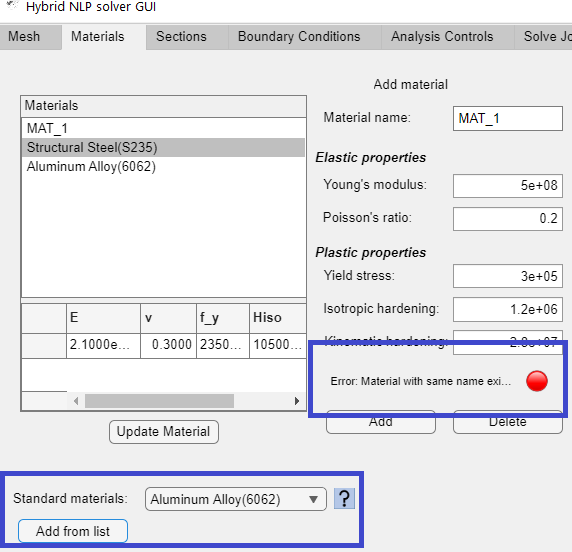
\includegraphics[scale=0.6]{GUIpics/TAB2/TAB2_adding_already_predefmat.png}
	\caption{Error when trying to add a standard material that was already 
	added previously.}
	\label{fig:TAB2_adding_already_predefmat}
\end{figure}

\section{The Sections tab}

The third tab pertains to cross-section defintion. Cross-sections as objects 
are assigned a name, a shape, numeric values pertaining to the basic dimension 
of the selected shape (e.g. two basic dimensions for rectangular sections). 
Moreover, each section is assigned a material. As a consequence the 
\textit{Sections} tab has a dependency on the \textit{Materials} tab. If a  
material gets deleted, then all sections that were assigned that material get 
deleted as well. 

We now proceed with the description of the essential parts of the 
\textit{Sections} tab, shown in Fig. \ref{fig:TAB3_marked}.

\begin{itemize}
	\item \textbf{A}: The \textit{Sections} tab.
	\item \textbf{B}: Here, the user assign a name and a shape to the section. 
	The name field takes alphanumeric values. If not specified, then the name 
	\textbf{Section\_}$\#$ is assigned to the section, where $\# = 1,2,3, ...$. 
	The available shapes from the drop-down list are i) rectangular and ii) 
	(symmetric) wide flange geometries. 
	\item \textbf{C}: In this section, the user assigns numeric values to the 
	relevant fields that pertain to the basic dimensions of the assigned shape. 
	A rectangular shape has to basic dimensions: height $h$ and width $b$. The 
	wide flange shape has 2 additional shapes: web thickness $t_w$ and flange 
	thickness $t_f$. In addition, the user also specifies which material will 
	be assigned to the section. As can be seen from Fig. 
	\ref{fig:TAB3_section_added}, the section \textbf{Rectangular\_Section} is 
	assigned the material \textbf{MAT\_1} defined previously. The drop-down 
	list is also shown, where all other materials defined in the 
	\textit{Materials} tab are available in the list.
	\item \textbf{D}: Axes that depict the cross-section shape selected from 
	the drop-down list. The basic dimensions are also indicated in each case.
	\item \textbf{E}: In this part, the user assigns sections to elements. 
	Tapered element capabilities are not included in the present code, therefor 
	only one section per element is permitted. A section is selected from the 
	\textit{Cross-Sections} panel, which is located at the top left of the tab 
	(see also \textbf{Item G} below) and then an element has to be selected 
	that will be assigned the section. Another feature for this part is the 
	capability to assign a specific to all elements, which is done by selecting 
	a section and then clicking on the \textit{Assign to all elements} button. 
	Lastly, a Success/Error indicator is included here as well in order to 
	facilitate the assignment process. For elements that are successfully 
	assigned a section, a message will be shown that states the name of the 
	assigned section, as shown in Fig. \ref{fig:TAB3_section_assigned} for 
	\textbf{Element 1} which was assigned the section 
	\textbf{Aluminum\_Section}. In contrast, for elements that have not been 
	assigned a section, when selected in the drop-down list, the indicator will 
	turn red and an appropriate message will be displayed. This can be seen in 
	Fig. \ref{fig:TAB3_NOsection_assigned}.
\end{itemize}

\begin{figure}
	\centering
	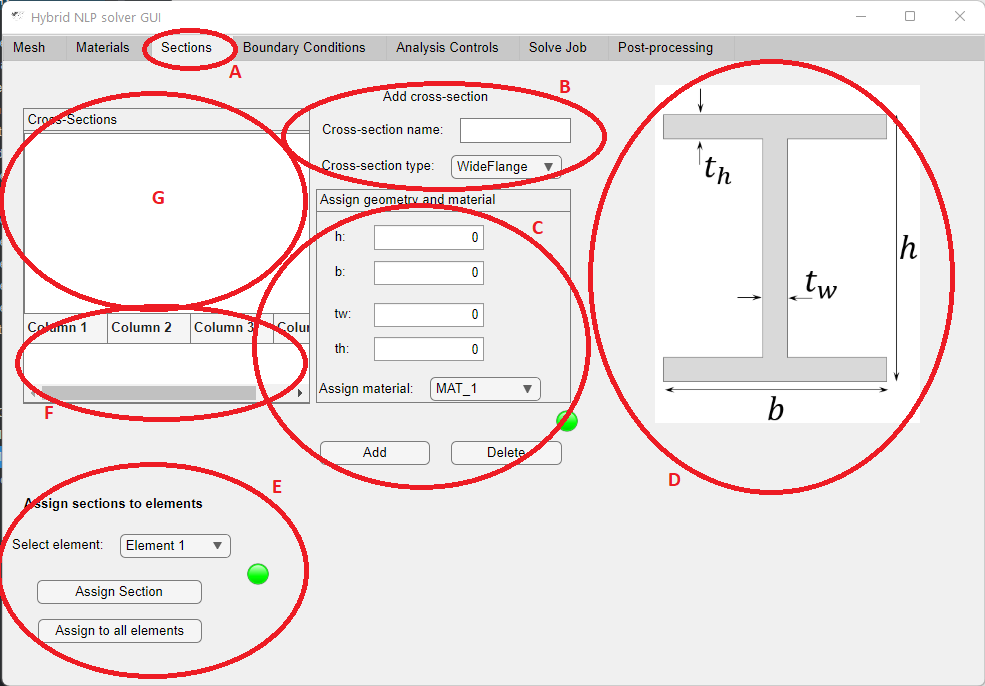
\includegraphics[scale=0.6]{GUIpics/TAB3/TAB3_marked.png}
	\caption{The \textit{Sections} tab with all essential parts marked in red 
		cycles and enumerated.}
	\label{fig:TAB3_marked}
\end{figure}

\begin{itemize}
	\item \textbf{F}: Table that lists the basic dimensions for the section 
	currently under selection in the \textit{Cross-Sections} panel (see below).
	\item \textbf{G}: The \textit{Cross-Sections} panel is where all sections 
	created are listed. In order to delete or assign a section to an element, 
	it has to be selected from the panel. 
\end{itemize}
\clearpage
\begin{figure}[t]
	\centering
	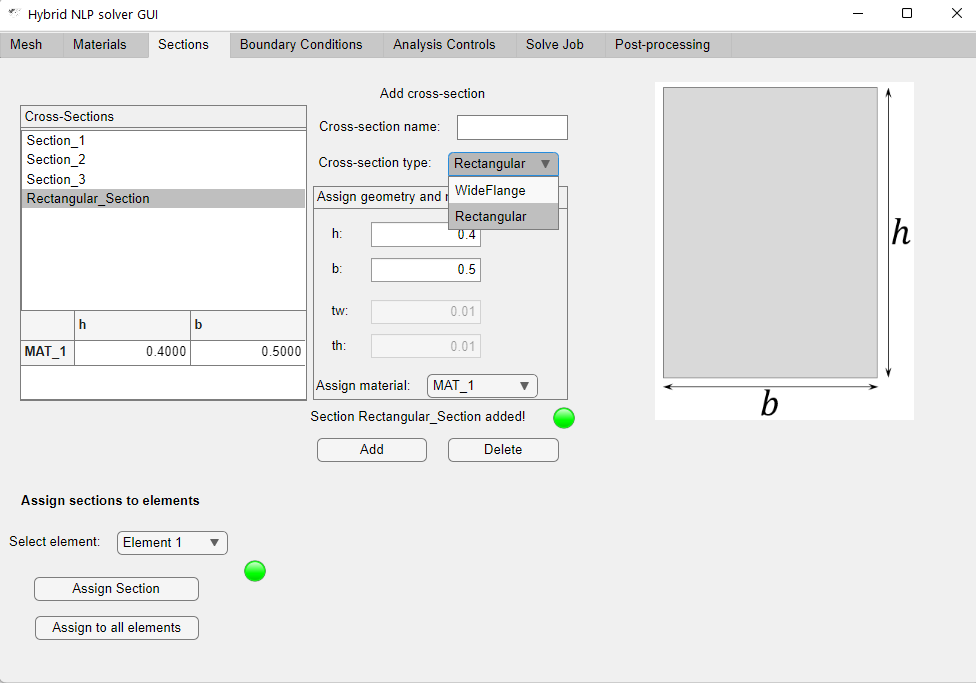
\includegraphics[scale=0.5]{GUIpics/TAB3/TAB3_section_added.png}
	\caption{Typical section definition process. A previously defined material 
	\textbf{MAT\_1} is assigned to section \textbf{Rectangular\_Section}.}
	\label{fig:TAB3_section_added}
\end{figure}

\begin{figure}[b]
	\centering
	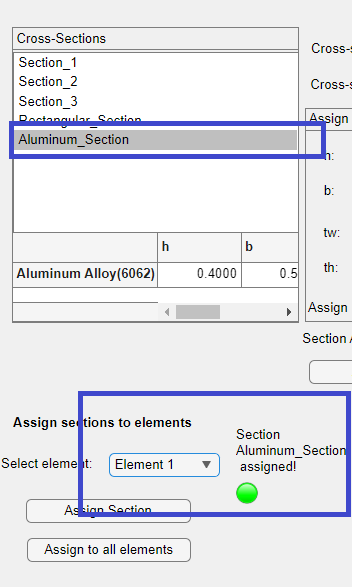
\includegraphics[scale=0.5]{GUIpics/TAB3/TAB3_section_assigned.png}
	\caption{Successful section assignment for \textbf{Element 1}.}
	\label{fig:TAB3_section_assigned}
\end{figure}
\clearpage
\begin{figure}
	\centering
	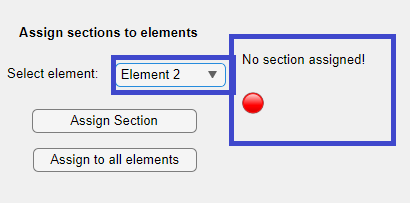
\includegraphics[scale=0.6]{GUIpics/TAB3/TAB3_NOsection_assigned.png}
	\caption{Indication that \textbf{Element 2} still needs to be assigned a 
	cross-section.}
	\label{fig:TAB3_NOsection_assigned}
\end{figure}


